\onecolumn

\appendix
\appendixpage
\addappheadtotoc
% \appendix
\setlength{\voffset}{-0.75in}
\addtolength{\textheight}{0.75in}
% \part*{Appendices}
% \addcontentsline{toc}{chapter}{Appendices}



% \setcounter{chapter}{0}

\renewcommand{\thesection}{\Alph{section}}

\section{FMEA risk analysis}\label{appendix:fmea}
\begin{table}[h!]
\begin{tabularx}{\textwidth}{|p{3.5em}|X|X|p{1em}|p{1em}|p{1em}|p{1.5em}|X|} \hline
    \rowcolor{tablegrey}
    Process Step & Potential Failure Mode & Potential \mbox{Effects} & S & O & D & RPN & C \\\hhline{========}
    CUDA integration & Codegen changes not available & Changes made to integrate CUDA with GPI not upstreamed later & 6 & 4 & 3 & 72 & Delay CUDA integration untill codegen is available\\\cline{3-8}
    && CUDA integration not completed & 6 & 5 & 4 & 90 & Go ahead with old codegen if new codegen is unavailable\\\hline
    Halo Exchange & Synchronisation issues & Incorrect data values used in computation & 8 & 5 & 2 & 80 & Validate results on many test applications against sequential OP2\\\hline
    Compute loop & Poor Performance & Causes simulations to run slower than the MPI version & 4 & 5 & 2 & 40 & Compare performance to MPI at every stage\\\hline
    Memory layout optimisations & Changes invalidating previous work & Setting back project timeline & 5 & 6 & 3 & 90 & Abstract the base data access to reduce work needed if data format changes\\\hline
    Testing & Incomplete test coverage & An error is present in the final system & 7 & 5 & 6 & 210 & Ensure multiple team members look over each section of work\\\hline
    Perfor-mance analysis & No access to system that supports RDMA (i.e. infiniband)& Inaccurate performance evaluation & 4 & 6 & 4 & 96 & Compare with MPI on available systems\\\hline
\end{tabularx}
\end{table}

\newpage
\section{Initial Gantt Chart}\label{appendix:Gantt_chart_original}
\begin{figure}[h!]
    \centering
    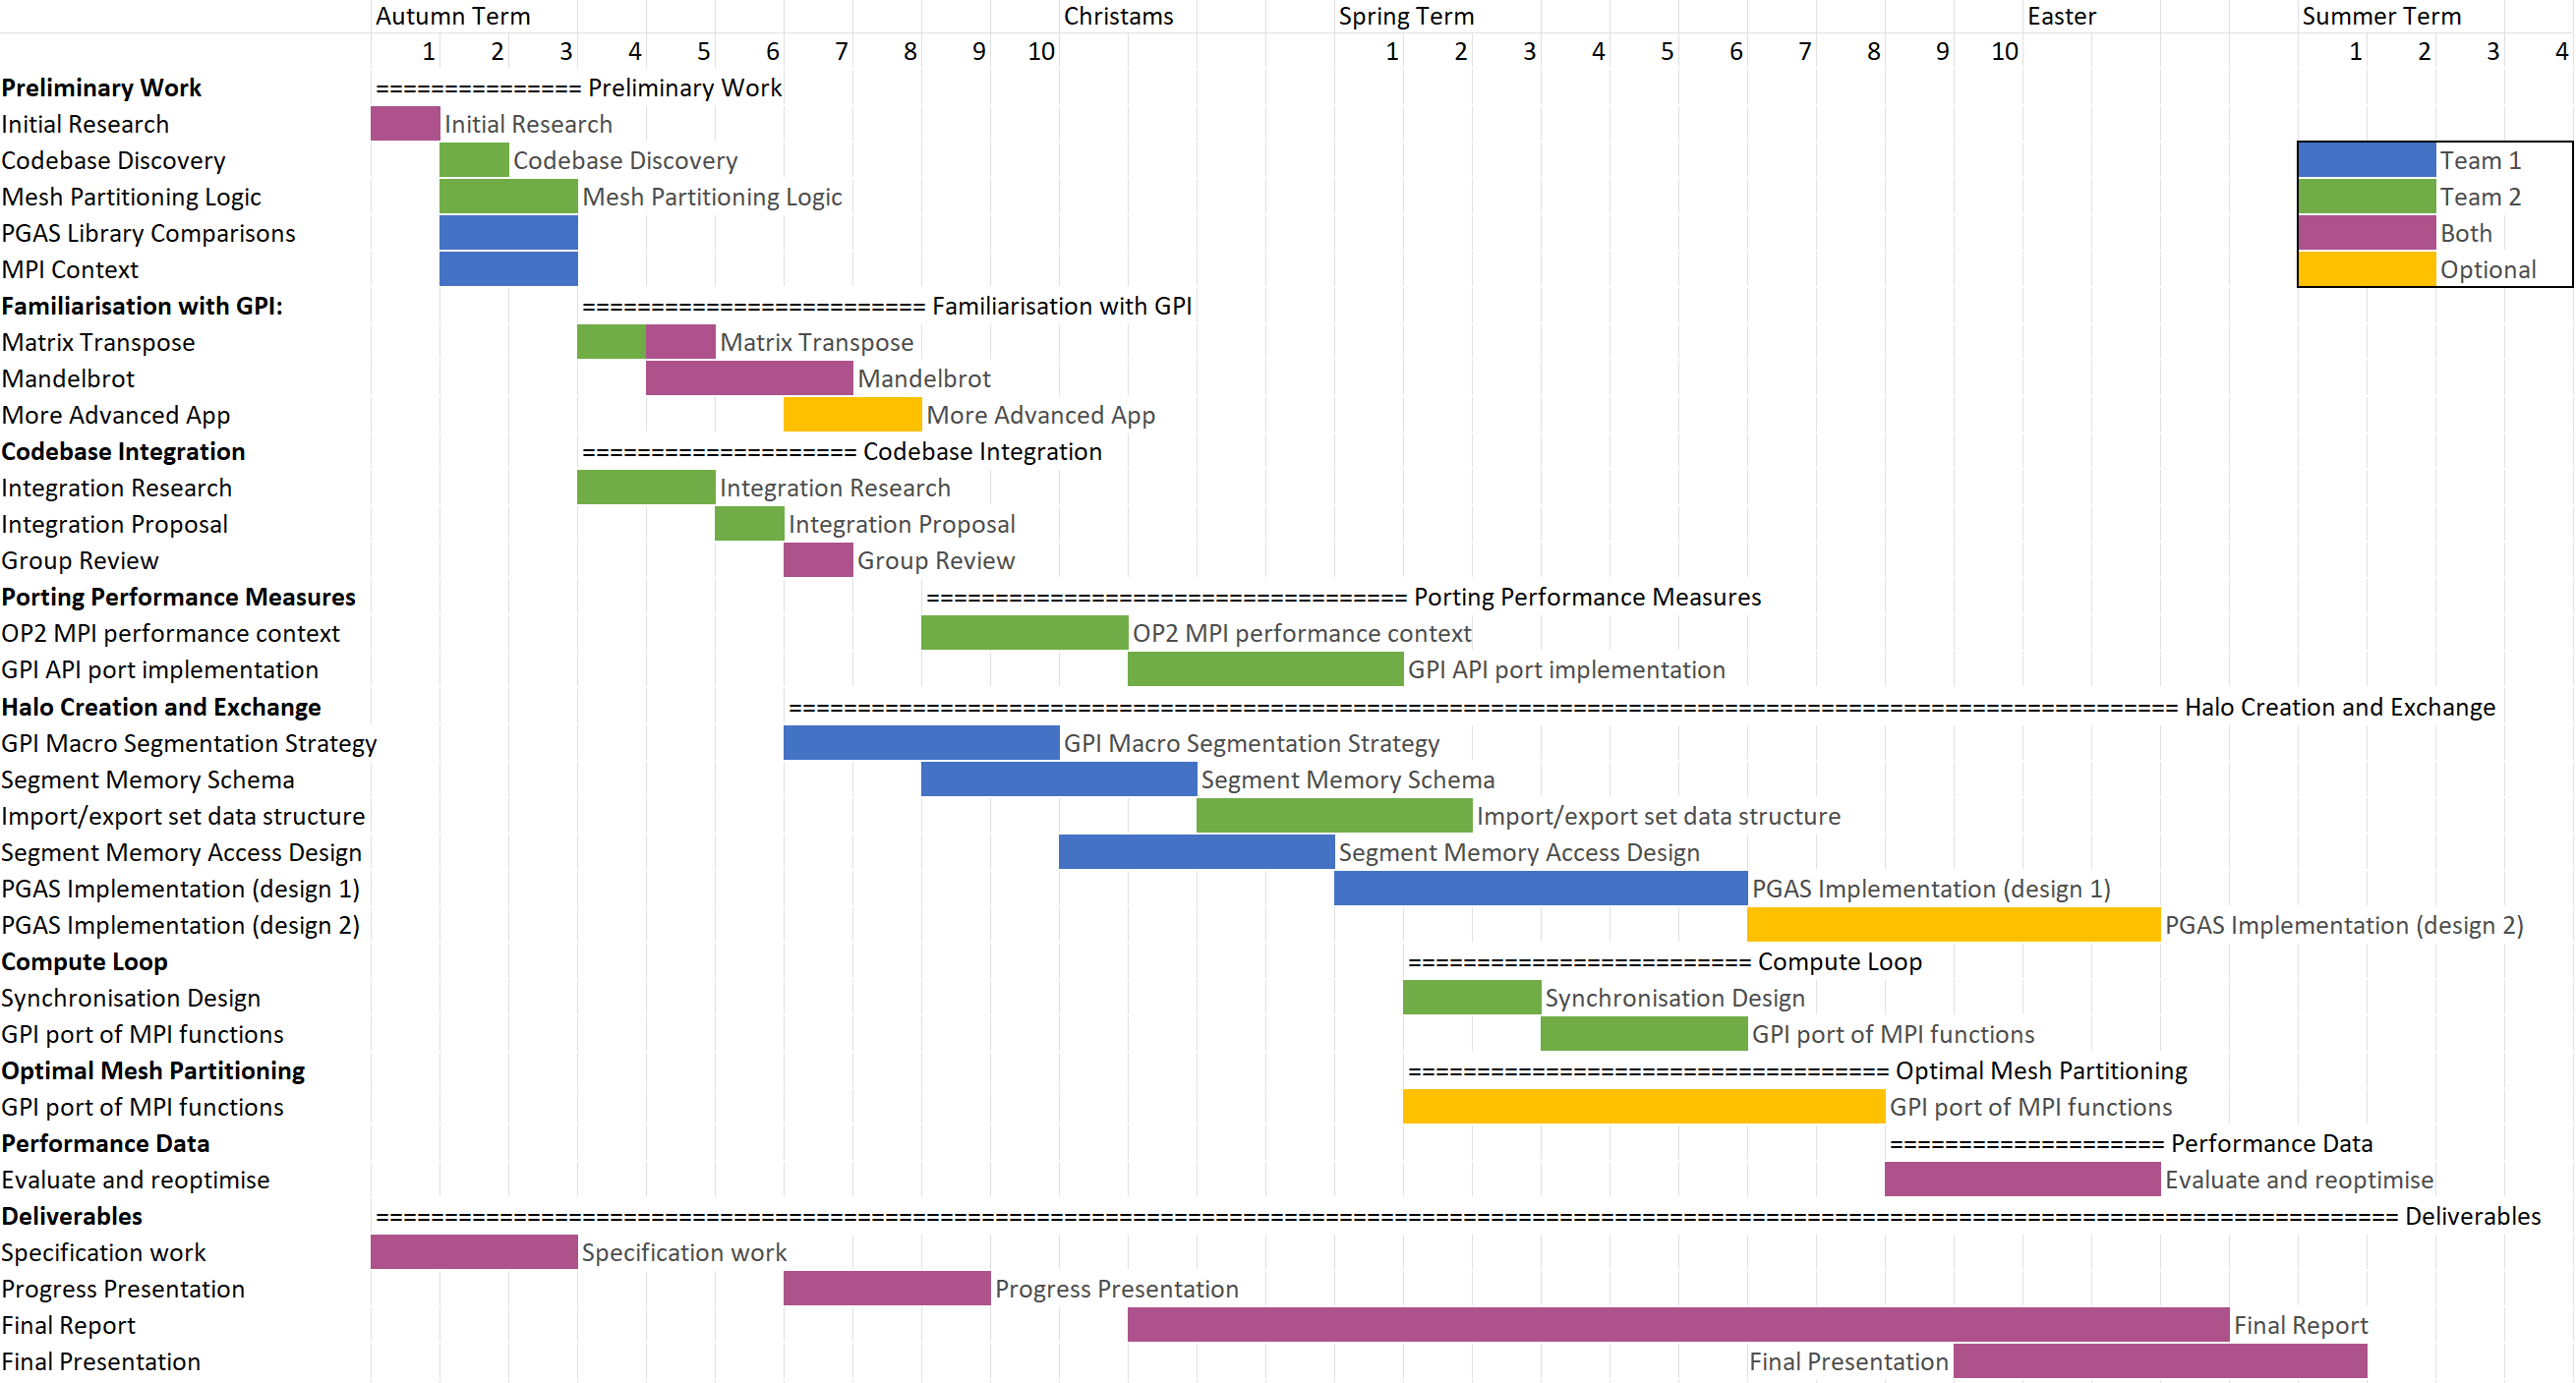
\includegraphics[width=0.8\textheight, angle=90]{figures/Gantt_Chart_Original.png}
    %\caption{Original Gantt Chart}
\end{figure}

\newpage
\section{Final Gantt Chart}\label{appendix:Gantt_chart_new}
\begin{figure}[h!]
    \centering
    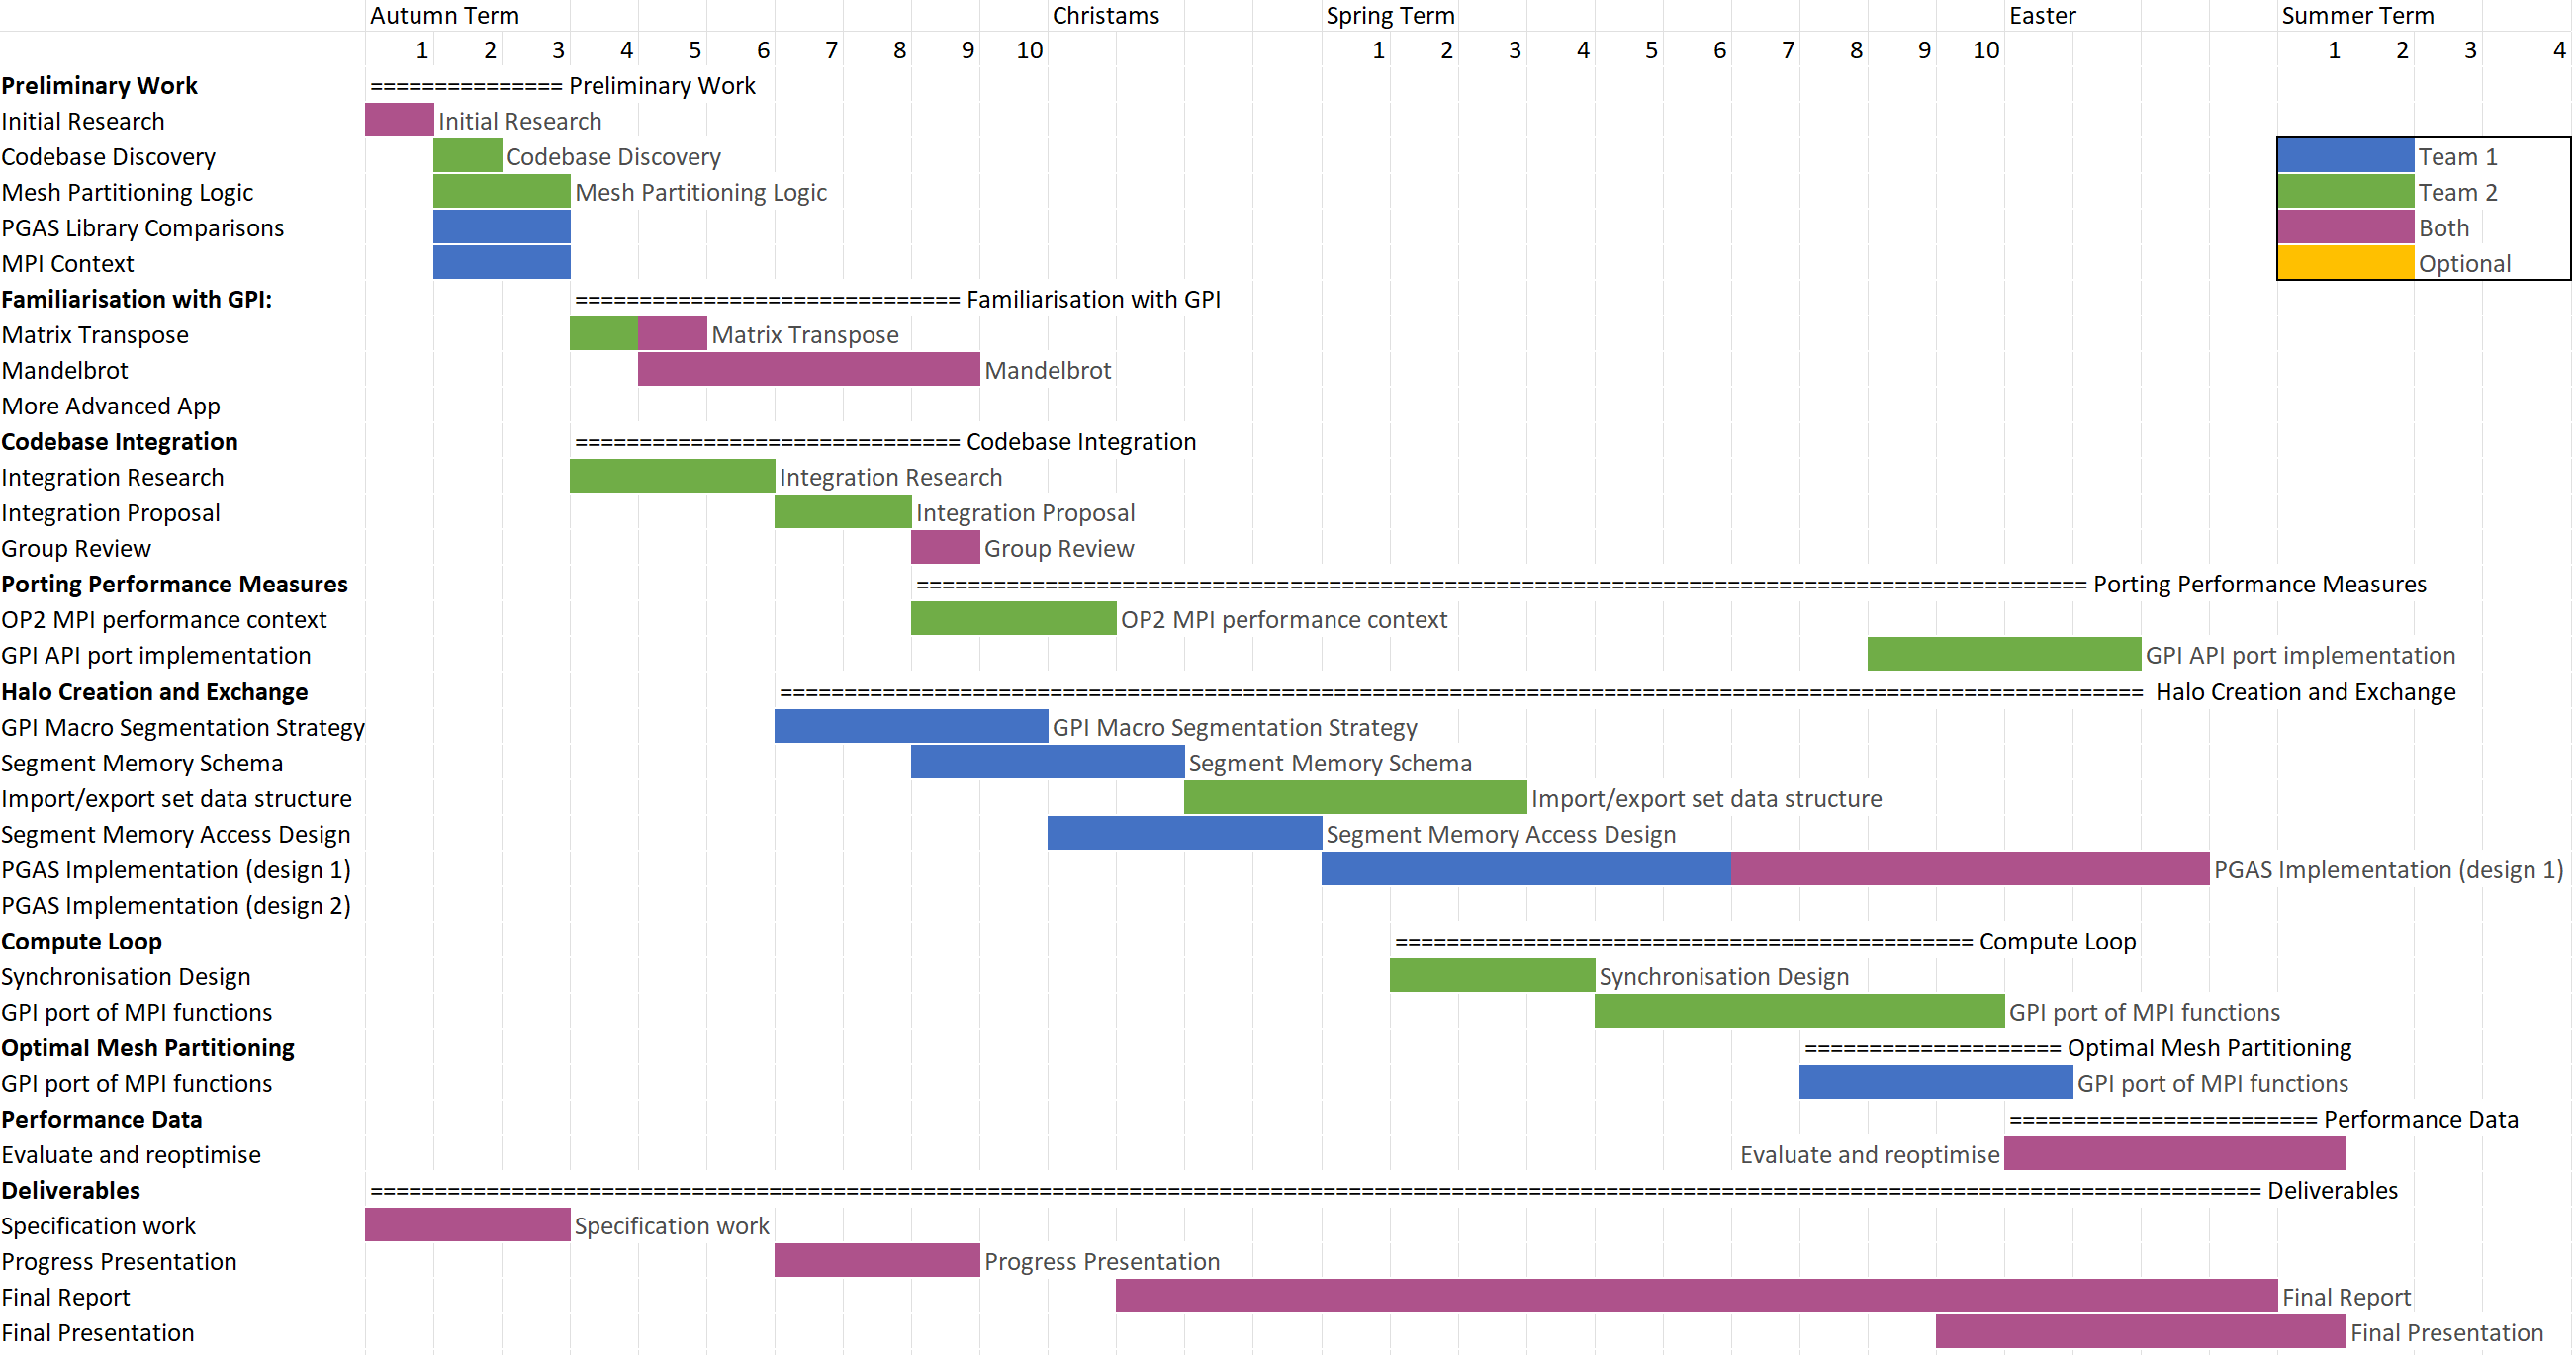
\includegraphics[width=0.8\textheight, angle=90]{figures/Gantt_Chart_New.png}
\end{figure}

